\subsection{WebApp - BackEnd}\label{sec:WebAppBackEnd}
WebApp - BackEnd is a Middleware that runs on the server. This Middleware (server-side software) facilitates client-server connectivity, forming a middle layer between the app(s) and the network: the server, the database, the operating system, and more. It receives requests from the clients (in this case, the WebApp - FrontEnd) and contains the logic to send the appropriate data back to the applicant over HTTP and REST.  These are the main conventions that provide structure to the request-response cycle between clients and servers.

WebApp - BackEnd is an application built with Node.js, an application platform where developers can write Javascript programs compiled, optimized, and interpreted by the V8 virtual machine. Node.js can create quick, reliable websites and products in a much efficient manner. Developing easy-to-scale real-time applications in other technologies is a bit difficult, but JavaScript technologies made it  more accessible.

The WebApp - BackEnd is composed of the API Gateway, Service Layer, and Resource Locator, more detailed below.

\subsubsection{API Gateway}\label{sec:APIGateway}
API Gateway is a managed service that enables easy  creation, publish, maintain, monitor, and secure REST APIs to act as a "gateway" for applications to access data, business logic, or functionality in the backend services, such as workloads. The API Gateway provides a simple uniform view of external resources to the internals of this application. It manages all tasks involved in receiving and processing API calls, including traffic management, authorization and access control, and monitoring and managing API versions.

\begin{figure}[htbp]
\begin{center}
  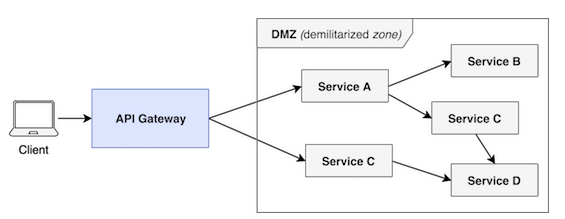
\includegraphics[scale=0.75]{images/apigateway.png}
\caption{API Gateway.}
\label{default-regular2}
\end{center}
\end{figure}

Basically, the gateway is an interface that receives calls to its internal systems, being a large gateway. It acts in five different ways:

\begin{itemize}
\item Filter for call traffic from different media;
\item A single gateway to the various API's that are exposed;
\item Router: API and Rate Limit traffic router;
\item Security engine with authentication and logging.
\end{itemize}

Gateway access can be done from many different devices. Therefore, it must have the power to unify outgoing calls and deliver to the user content that can be accessed from any browser and system. In this project, the gateway interaction happens with the frontend web app. The Gateways as a Security Feature: In the APIs world, one of the most subjects talked about issues is always security, and having an API Gateway is one of the best solutions on the market to get complete control of API's, because this pattern addresses the so-called CIA (Confidentiality, Integrity, Availability) almost flawlessly.

\subsubsection{Service Layer}\label{sec:ServiceLayer}
A Service Layer defines an application's boundary and its set of available operations from the perspective of interfacing client layers. It encapsulates the application's business logic, controlling transactions and coordinating responses in the implementation of its operations.

Enterprise applications typically require different interfaces to the data they store and the logic they implement: data loaders, user interfaces, integration gateways, and others. Despite their different purposes, these interfaces often need common interactions with the application to access and manipulate its data and invoke its business logic. The interactions may be complex, involving transactions across multiple resources and coordinating several responses to an action. Encoding the logic of the interactions separately in each interface causes much duplication. The service layer provides:

\begin{enumerate}
\item Centralizes external access to data and functions.
\item Hides (abstracts) internal implementation and changes.
\item Allows for versioning of the services.
\end{enumerate}

The service layer acts as an orchestrator, controlling the flow of incoming and outcoming information requests and responses. Orchestration allows to directly link process logic to service interaction within workflow logic. This combines a business process model with service-oriented modeling and design, realizing workflow management through a process service model. Orchestration brings the business process into the service layer, positioning it as a master composition controller.

\subsubsection{Resource Locator}\label{sec:ResourceLocator}

Resource locators are components that abstract the persistence layer. Their job is to provide an object that can help services discover and persist information from/to the Data Storage Module. Information can be stored in the Blockchain, Filesystem, or Database, and resource locators should know precisely where to get/put data within them.  